\chapter{Results and Tests}
\label{chap:results}

\section{Energy efficiency}
Using the Energy monitoring tool we observed the board idling on a power consumption level of about $2.0 \mu A$ while running the final iteration of the program with sleep mode enabled.

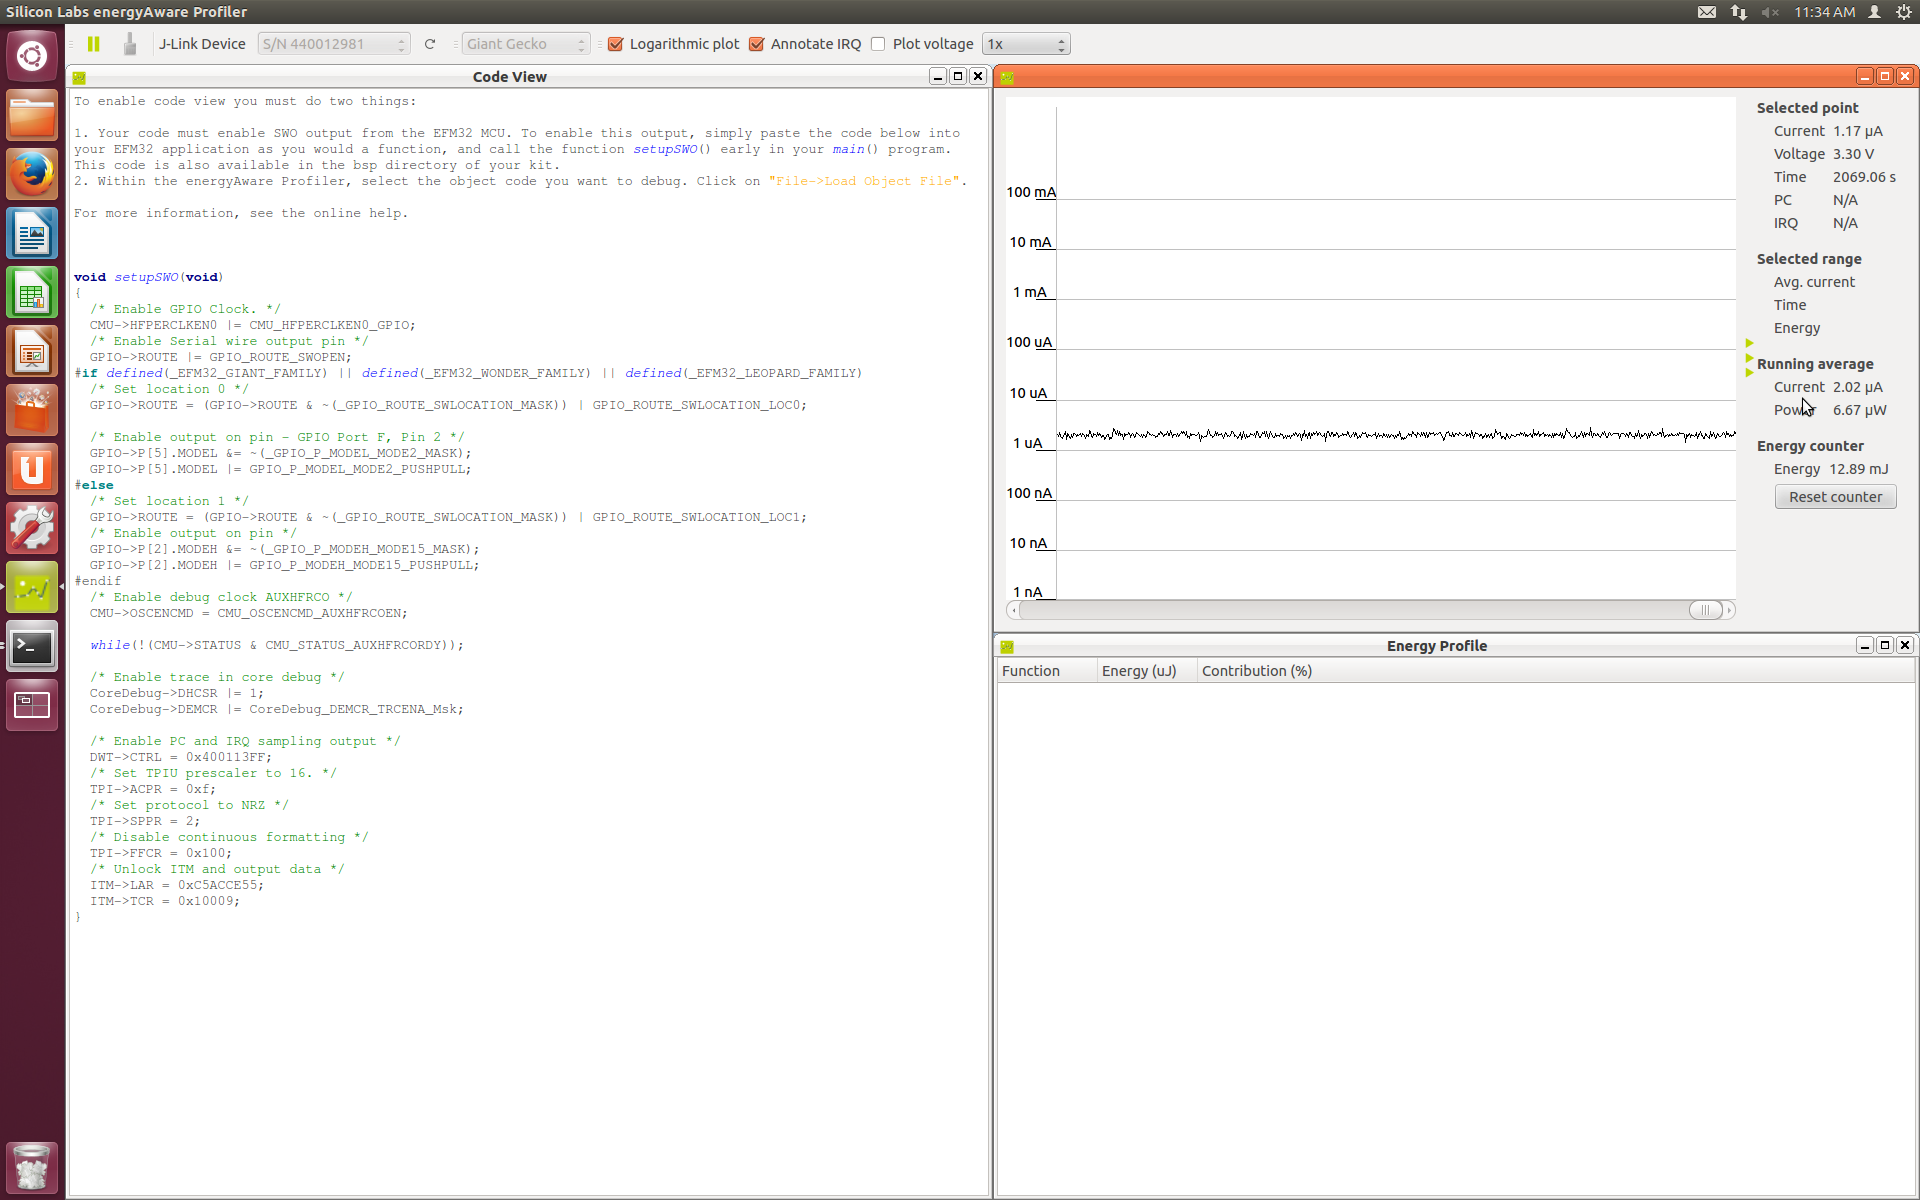
\includegraphics[width=\linewidth]{img/eAProfiler.png}

Representatives from Silicon Labs, the manufacturer of the EFM32GG STK have used the cr2032 "coin cell" battery as an example when talking about the enery efficiency of their products. For this reason we chose to look up some statistics about this battery online and use them to calculate the theoretical time the development board can run on one battery. One battery manufacturer claims [http://www.cr2032.co/cms/prodimages/energizer\_cr2032\_datasheet.pdf] their battery has a typical capacity of $240 mAh$.

\[
	240 mAh / 2.0 uA = 120 000 hours = 5000 days = 13.7 years
\]

According to one source \cite{cr2032} a coin cell battery can last up to 5 years while in use before deteriorating too much. In other words the battery will deteriorate before discharging from use for this microcontroller running this sleeping program.

\section{Tests}
Testing was not emphasised in this exercise. The final version of the program features a simple button-to-LED mapping that can be tested by simply pushing one or more buttons and observing the lights.

\section{Discussion}
The primary goal of the exercise was learning, and that was definently achieved. The group members had no significant prior experience with the technologies, only some theoretical knowledge from the TDT4160 course. But thanks to the instructions in the compendium we were able to do most of the work on our own.

The biggest problem we had was enabling sleep mode with interrupt-based I/O. After following the instructions in the compendium we had sucessfully implemented the I/O with interrupts, but the microcontroller did not go to sleep mode. Attempts at debugging revealed that removing code crucial to the I/O made the device go to sleep. It seemed impossible to solve the problem, but inexplicably it suddenly began working after moving some code about, even though it seems that should not have changed anything.
